% Options for packages loaded elsewhere
\PassOptionsToPackage{unicode}{hyperref}
\PassOptionsToPackage{hyphens}{url}
\documentclass[
  12pt,
  ignorenonframetext,
  aspectratio=169]{beamer}
\newif\ifbibliography
\usepackage{pgfpages}
\setbeamertemplate{caption}[numbered]
\setbeamertemplate{caption label separator}{: }
\setbeamercolor{caption name}{fg=normal text.fg}
\beamertemplatenavigationsymbolsempty
% remove section numbering
\setbeamertemplate{part page}{
  \centering
  \begin{beamercolorbox}[sep=16pt,center]{part title}
    \usebeamerfont{part title}\insertpart\par
  \end{beamercolorbox}
}
\setbeamertemplate{section page}{
  \centering
  \begin{beamercolorbox}[sep=12pt,center]{section title}
    \usebeamerfont{section title}\insertsection\par
  \end{beamercolorbox}
}
\setbeamertemplate{subsection page}{
  \centering
  \begin{beamercolorbox}[sep=8pt,center]{subsection title}
    \usebeamerfont{subsection title}\insertsubsection\par
  \end{beamercolorbox}
}
% Prevent slide breaks in the middle of a paragraph
\widowpenalties 1 10000
\raggedbottom
\AtBeginPart{
  \frame{\partpage}
}
\AtBeginSection{
  \ifbibliography
  \else
    \frame{\sectionpage}
  \fi
}
\AtBeginSubsection{
  \frame{\subsectionpage}
}
\usepackage{iftex}
\ifPDFTeX
  \usepackage[T1]{fontenc}
  \usepackage[utf8]{inputenc}
  \usepackage{textcomp} % provide euro and other symbols
\else % if luatex or xetex
  \usepackage{unicode-math} % this also loads fontspec
  \defaultfontfeatures{Scale=MatchLowercase}
  \defaultfontfeatures[\rmfamily]{Ligatures=TeX,Scale=1}
\fi
\usepackage{lmodern}
\usetheme[]{Madrid}
\ifPDFTeX\else
  % xetex/luatex font selection
\fi
% Use upquote if available, for straight quotes in verbatim environments
\IfFileExists{upquote.sty}{\usepackage{upquote}}{}
\IfFileExists{microtype.sty}{% use microtype if available
  \usepackage[]{microtype}
  \UseMicrotypeSet[protrusion]{basicmath} % disable protrusion for tt fonts
}{}
\makeatletter
\@ifundefined{KOMAClassName}{% if non-KOMA class
  \IfFileExists{parskip.sty}{%
    \usepackage{parskip}
  }{% else
    \setlength{\parindent}{0pt}
    \setlength{\parskip}{6pt plus 2pt minus 1pt}}
}{% if KOMA class
  \KOMAoptions{parskip=half}}
\makeatother
\setlength{\emergencystretch}{3em} % prevent overfull lines
\providecommand{\tightlist}{%
  \setlength{\itemsep}{0pt}\setlength{\parskip}{0pt}}
\usepackage{cancel}
\usepackage{tikz}
\usetikzlibrary{positioning,calc,arrows.meta}
\tikzset{>={Stealth[length=3mm,width=2mm]}}
\definecolor{UBCblue}{rgb}{0.04706, 0.13725, 0.26667}
\usecolortheme[named=UBCblue]{structure}
\setbeamertemplate{frametitle}{\color{UBCblue}\bfseries\insertframetitle\par\vskip-6pt\hrulefill}
\setbeamercolor{title in head/foot}{bg=white,fg=gray}
\setbeamercolor{section in head/foot}{bg=white,fg=gray}
\setbeamercolor{author in head/foot}{bg=white,fg=gray}
\setbeamercolor{date in head/foot}{bg=white,fg=gray}
\setbeamertemplate{page number in head/foot}{}
\setbeamertemplate{frame numbering}[none]
\setbeamercolor{alerted text}{bg=yellow}
\AtBeginSection[]{\begin{frame}\frametitle{Today's lecture}{\Large\tableofcontents[currentsection]}\end{frame}}
\makeatletter
\def\ps@titlepage{%
  \setbeamertemplate{footline}{}
}
\addtobeamertemplate{title page}{\thispagestyle{titlepage}}{}
\makeatother
\include{toc}
\usepackage{bookmark}
\IfFileExists{xurl.sty}{\usepackage{xurl}}{} % add URL line breaks if available
\urlstyle{same}
\hypersetup{
  pdftitle={How can we formulate our research questions effectively?},
  pdfauthor={Yongjin Park},
  hidelinks,
  pdfcreator={LaTeX via pandoc}}

\title{\texorpdfstring{How can we formulate our research questions
effectively?}{How can we formulate our research questions effectively?}}
\author{\texorpdfstring{Yongjin Park}{Yongjin Park}}
\date{13 January 2026}

\begin{document}
\frame{\titlepage}

\begin{frame}{Course Logistics}
\protect\phantomsection\label{course-logistics}
\begin{columns}[T]
\begin{column}{.2\linewidth}
\end{column}

\begin{column}{.7\linewidth}
\Large

\textbf{Please fill out the survey}

of your background
\end{column}
\end{columns}
\end{frame}

\begin{frame}{Advertisement}
\protect\phantomsection\label{advertisement}
\Large

\begin{itemize}
\tightlist
\item
  \href{https://asda.stat.ubc.ca/}{ASDA}
\end{itemize}

\normalsize

\begin{itemize}
\item
  \url{https://asda.stat.ubc.ca/2025/11/10/free-stats-help.html}
\item
  If you and your team are interested in the following ASDA projects,
  let me know.
\item
  I will send you one-page project proposal document.
\end{itemize}
\end{frame}

\begin{frame}{ASDA \#1: Blood RNAs for Febrile Illness Diagnosis}
\protect\phantomsection\label{asda-1-blood-rnas-for-febrile-illness-diagnosis}
\begin{itemize}
\item
  Scoping review identified 286 RNA signatures from literature
\item
  Signatures diagnose or predict outcomes of febrile illnesses (sepsis,
  TB, infections)
\item
  Goal: Characterize and understand potential sources of biases
\item
  Meta-analysis across many different studies
\end{itemize}
\end{frame}

\begin{frame}{ASDA \#2: \texttt{Breath\ print} data for Lung Cancer
Detection}
\protect\phantomsection\label{asda-2-breath-print-data-for-lung-cancer-detection}
\begin{itemize}
\item
  Breath samples from 500+ participants (lung cancer vs.~healthy
  controls)
\item
  Volatile organic compounds (VOCs) analyzed via mass spectrometry
\item
  High-dimensional data: \textasciitilde500-1500 compounds per sample
\item
  Goal: Build analysis pipeline for biomarker discovery and
  classification
\end{itemize}
\end{frame}

\begin{frame}{Roadmap of STAT/BIOF/GSAT540 2026}
\protect\phantomsection\label{roadmap-of-statbiofgsat540-2026}
\emph{data generation} followed by \emph{inference} or validation

\vfill

\large

\begin{columns}[T]
\begin{column}{.45\linewidth}
\begin{enumerate}
\setcounter{enumi}{1}
\item
  \emph{Statistics and matrix algebra}
\item
  \textbf{\color{magenta}Formulating biological questions} (Today)
\item
  \textbf{\color{teal} Hypothesis testing} (Thursday)
\item
  RNA-seq data analysis
\item
  Statistical inference
\end{enumerate}
\end{column}

\begin{column}{.45\linewidth}
\begin{enumerate}
\setcounter{enumi}{7}
\item
  Single-cell genomics
\item
  Matrix factorization
\item
  Genome-wide association studies
\item
  Multiple hypothesis testing
\end{enumerate}
\end{column}
\end{columns}

\normalsize
\end{frame}

\begin{frame}{}
\protect\phantomsection\label{section}
\huge

A biological problem \(\implies\)

\flushright

a computational problem

\normalsize
\end{frame}

\begin{frame}{Guide 1: Crystallize abstract ideas into a concrete
computational problem by writing a paper}
\protect\phantomsection\label{guide-1-crystallize-abstract-ideas-into-a-concrete-computational-problem-by-writing-a-paper}
\begin{columns}[T]
\begin{column}{.45\linewidth}
\begin{block}{Research Model \#1}
\protect\phantomsection\label{research-model-1}
\begin{enumerate}
\tightlist
\item
  Idea
\item
  Do research
\item
  Write a paper
\end{enumerate}
\end{block}
\end{column}

\begin{column}{.45\linewidth}
\begin{block}{Research Model \#2}
\protect\phantomsection\label{research-model-2}
\begin{itemize}
\tightlist
\item
  Idea
\item
  \textbf{Write a paper}
\item
  Do research
\end{itemize}
\end{block}
\end{column}
\end{columns}

Which model would work better for you? Why?

\only<2>{
${}$
\centerline{\textbf{\color{teal} Discussion with your peers around you (5 min).}}
${}$
}

\vfill

\normalsize

\begin{enumerate}
\item<3-> Model \#2 forces us to be clear, focused
\item<3-> Crystallizes what we don’t understand yet (and what we don't need to know)
\item<3-> Opens the way to dialogue with others: reality check and collaboration
\end{enumerate}

\tiny

Simon Peyton Jones,
\href{https://www.microsoft.com/en-us/research/wp-content/uploads/2016/07/How-to-write-a-great-research-paper.pdf}{How
to write a great research paper}

\normalsize
\end{frame}

\begin{frame}{}
\protect\phantomsection\label{section-1}
\huge
\begin{center}
${}$ Model \#1 or \#2?
\end{center}
\end{frame}

\begin{frame}{Guide 2: Ten simple rules \ldots{}}
\protect\phantomsection\label{guide-2-ten-simple-rules}
\begin{columns}[T]
\begin{column}{.3\linewidth}
\end{column}

\begin{column}{.66\linewidth}
\large

William Noble,

\href{https://journals.plos.org/ploscompbiol/article?id=10.1371/journal.pcbi.1010786}{\textbf{Ten
simple rules for defining a computational biology project.}}

\emph{PLoS Comput Biol} (2023)

\normalsize
\end{column}
\end{columns}
\end{frame}

\begin{frame}{Summary: Ten Simple Rules}
\protect\phantomsection\label{summary-ten-simple-rules}
\large

\begin{columns}[T]
\begin{column}{.43\linewidth}
\begin{enumerate}
\tightlist
\item
  \textbf{\color{teal} Write it down}
\item
  \textbf{\color{teal} Define the problem}
\item
  Define potential impact
\item
  Summarize related work
\item
  \textbf{\color{teal} State central hypothesis}
\end{enumerate}
\end{column}

\begin{column}{.47\linewidth}
\begin{enumerate}
\setcounter{enumi}{5}
\tightlist
\item
  Sketch your approach
\item
  \textbf{\color{teal} Identify available data}
\item
  Choose validation measures
\item
  Set up version control
\item
  Share with colleagues
\end{enumerate}
\end{column}
\end{columns}

\normalsize

\[{}\]

\textbf{\color{blue}\large Discussion: How many items have you followed in the past?}
\end{frame}

\begin{frame}{Rule 1: Write it down}
\protect\phantomsection\label{rule-1-write-it-down}
\Large

Document your idea in ``writing''

\normalsize

\vfill

\begin{itemize}
\item
  Clarifies your thinking and the underlying problem
\item
  Exposes half-baked concepts early
\item
  Forces you to articulate assumptions
\end{itemize}

\begin{quote}
``The act of writing your idea down will inevitably clarify it for
you.''
\end{quote}

\vfill

\textbf{Even a rough draft is better than no draft}
\end{frame}

\begin{frame}{Rule 2: Define the problem}
\protect\phantomsection\label{rule-2-define-the-problem}
\Large

Clearly delineate the scope and nature of the problem

\normalsize

\vfill

\begin{itemize}
\item
  What exactly are you trying to solve?
\item
  What is \textbf{in scope} vs.~\textbf{out of scope}?
\item
  Be specific, not vague

  \begin{itemize}
  \tightlist
  \item
    ma\vfill
  \end{itemize}
\end{itemize}

Which sounds more specific?

\begin{columns}[T]
\begin{column}{.45\linewidth}
\begin{itemize}
\tightlist
\item
  Understand gene expression programs in myeloid cancer
\end{itemize}
\end{column}

\begin{column}{.45\linewidth}
\begin{itemize}
\tightlist
\item
  Predict enhancer-promoter interaction in K562 cells
\end{itemize}
\end{column}
\end{columns}
\end{frame}

\begin{frame}{Rule 4: Summarize related work}
\protect\phantomsection\label{rule-4-summarize-related-work}
\Large

Conduct literature review early

\normalsize

\vfill

\begin{quote}
``A terrible trap to fall into is carrying out an entire research
project only to find that the same work was already published before you
began.''
\end{quote}

\begin{itemize}
\item
  Learn from others' approaches
\item
  Identify gaps in current knowledge
\item
  \textbf{Summarize} methods in a chronologically ordered table
\end{itemize}
\end{frame}

\begin{frame}{Rule 5: State central hypothesis}
\protect\phantomsection\label{rule-5-state-central-hypothesis}
\Large

Reduce your idea to a single sentence

\large

\vfill

\begin{itemize}
\item
  Focus on the one, single, \textbf{overarching} theme
\item
  Make it \textbf{testable}
\item
  Keep it \textbf{simple and clear}
\end{itemize}

\vfill

\normalsize

\begin{itemize}
\tightlist
\item
  It takes practice and time.
\end{itemize}
\end{frame}

\begin{frame}{Rule 7: Identify available data}
\protect\phantomsection\label{rule-7-identify-available-data}
\Large

Ensure you have both inputs and validation data

\normalsize

\vfill

\begin{itemize}
\item
  What are the input?
\item
  How do we know that our discovery is correct?
\item
  Simulation studies are okay.
\end{itemize}
\end{frame}

\begin{frame}[fragile]{Rule 9: Set up version control}
\protect\phantomsection\label{rule-9-set-up-version-control}
\Large

Use \texttt{git} or a similar tool from day one

\normalsize

\vfill

\begin{itemize}
\item
  Track code evolution from project inception

  \begin{itemize}
  \tightlist
  \item
    Keep the dates
  \end{itemize}
\item
  Enable collaboration
\item
  Maintain reproducibility
\item
  Document your progress
\end{itemize}
\end{frame}

\begin{frame}{Rule 10: Share with colleagues}
\protect\phantomsection\label{rule-10-share-with-colleagues}
\Large

Seek feedback on feasibility and scientific importance

\normalsize

\vfill

\begin{itemize}
\item
  Prepare to ``Think Again'' (don't be embarrassed or offended by being
  wrong)
\item
  Refine your ideas through discussion
\item
  Find potential collaborators
\end{itemize}
\end{frame}

\begin{frame}{Ten Simple Rules (items) \(\to\) A paper}
\protect\phantomsection\label{ten-simple-rules-items-to-a-paper}
\begin{columns}[T]
\begin{column}{.43\linewidth}
\begin{enumerate}
\tightlist
\item
  \textbf{\color{teal} Write it down}
\item
  \textbf{\color{teal} Define the problem}
\item
  Define potential impact
\item
  Summarize related work
\item
  \textbf{\color{teal} State central hypothesis}
\item
  Sketch your approach
\item
  \textbf{\color{teal} Identify available data}
\item
  Choose validation measures
\item
  Set up version control
\item
  Share with colleagues
\end{enumerate}
\end{column}

\begin{column}{.47\linewidth}
\begin{itemize}
\tightlist
\item
  Abstract

  \begin{itemize}
  \tightlist
  \item
    Rule \#1, \#2, \#5
  \end{itemize}
\item
  Introduction

  \begin{itemize}
  \tightlist
  \item
    Rule \#2, \#3, \#4, \#5
  \end{itemize}
\item
  Results

  \begin{itemize}
  \tightlist
  \item
    Rule \#5, \#7, \#10
  \end{itemize}
\item
  Discussion

  \begin{itemize}
  \tightlist
  \item
    Rule \#10
  \end{itemize}
\item
  Methods

  \begin{itemize}
  \tightlist
  \item
    Rule \#6, \#7, \#8, \#9, \#10
  \end{itemize}
\end{itemize}
\end{column}
\end{columns}
\end{frame}

\begin{frame}{Bottom line}
\protect\phantomsection\label{bottom-line}
\Large

\({}\) \textbf{It's so critical to describe your problem clearly.}

\begin{itemize}
\item <2-> Recognize the underlying computational problem(s)
\item <3-> Make an actionable plan to solve them.
\item <4> Evaluate what/how it worked and didn't.
\end{itemize}
\end{frame}

\begin{frame}{Is defining a problem worth my time?}
\protect\phantomsection\label{is-defining-a-problem-worth-my-time}
\centerline{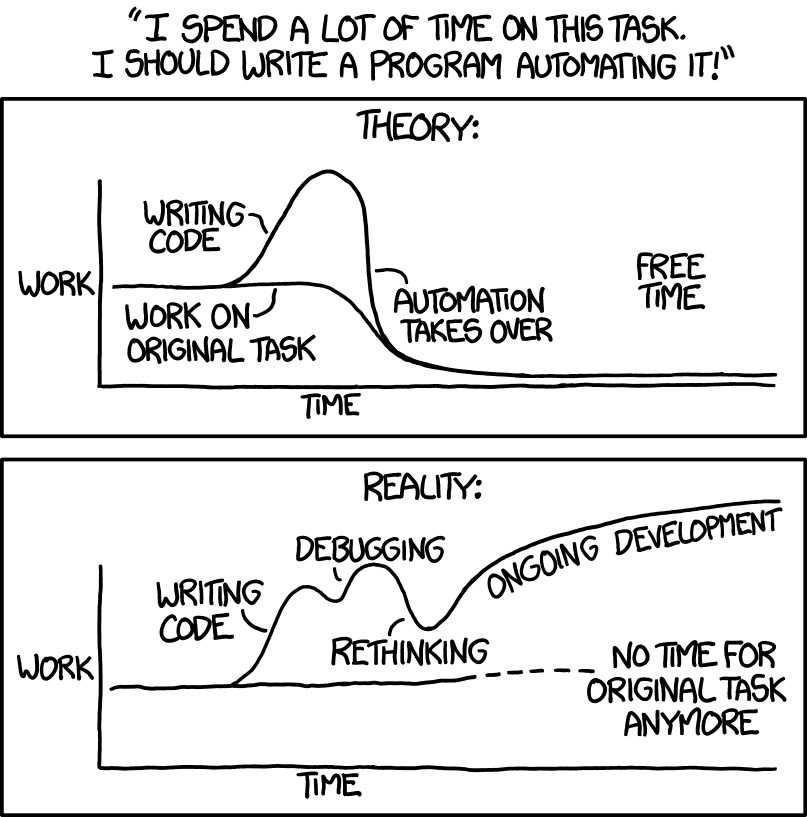
\includegraphics[height=.72\textheight]{img/automation_2x.png}}

\vfill

\tiny

\url{https://xkcd.com/1319/} \normalsize
\end{frame}

\begin{frame}{Two flavors}
\protect\phantomsection\label{two-flavors}
\begin{columns}[T]
\begin{column}{.45\linewidth}
\begin{itemize}
\item
  \#1: Optimization approach

  \begin{itemize}
  \item
    \textbf{\color{magenta} The art of abstraction}
  \item
    Define \textbf{input}, \textbf{output}, and \textbf{metric}
    (objective function)
  \item
    Find the same or similar existing problems in the literature
  \end{itemize}
\end{itemize}
\end{column}

\begin{column}{.45\linewidth}
\begin{itemize}
\item
  \#2: Probabilistic Modelling

  \begin{itemize}
  \item
    \textbf{ Think of a potential {\color{teal} generative model}}
  \item
    Describe the problem in terms of random variables
  \item
    Structural Equation Model (in epidemiology)
  \item
    Use an existing inference algorithm
  \end{itemize}
\end{itemize}
\end{column}
\end{columns}
\end{frame}

\section{Define a problem as an optimization
problem}\label{define-a-problem-as-an-optimization-problem}

\begin{frame}{The art of abstraction: Same data, different questions}
\protect\phantomsection\label{the-art-of-abstraction-same-data-different-questions}
\Large

Single-cell RNA-seq data: a matrix of \textbf{genes \(\times\) cells}

\normalsize

\vfill

Biological questions \(\rightarrow\) computational problems
\end{frame}

\begin{frame}{Exercise: Eleven Grand Challenges in Single-Cell}
\protect\phantomsection\label{exercise-eleven-grand-challenges-in-single-cell}
\footnotesize

Lähnemann et al., \emph{Genome Biology} (2020)

\normalsize

\begin{columns}[T]
\begin{column}{.48\linewidth}
\textbf{Transcriptomics}

\begin{enumerate}
\tightlist
\item
  Handling sparsity (dropout)
\item
  \textbf{\color{magenta} Defining cell identity}
\item
  Tracking cellular dynamics
\item
  Mapping to reference atlases
\end{enumerate}

\textbf{Genomics}

\begin{enumerate}
\setcounter{enumi}{4}
\tightlist
\item
  Finding variants (scDNA-seq)
\item
  Identifying copy-number changes
\item
  Inferring regulatory networks
\end{enumerate}
\end{column}

\begin{column}{.48\linewidth}
\textbf{Phylogenetics}

\begin{enumerate}
\setcounter{enumi}{7}
\tightlist
\item
  Understanding tumor evolution
\item
  Calling structural variants
\end{enumerate}

\textbf{Integration}

\begin{enumerate}
\setcounter{enumi}{9}
\tightlist
\item
  Multi-modal integration
\item
  Scaling to millions of cells
\end{enumerate}
\end{column}
\end{columns}

Let's work on one of these examples
\end{frame}

\begin{frame}{Example: Defining cell identity (Challenge 2)}
\protect\phantomsection\label{example-defining-cell-identity-challenge-2}
\Large

\textbf{Biological question:} What cell types are in my sample?

\vfill

\begin{itemize}
\item
  What are the variables of interest?
\item
  Is it important?
\end{itemize}

\normalsize
\end{frame}

\begin{frame}{How should we think of cells in this context?}
\protect\phantomsection\label{how-should-we-think-of-cells-in-this-context}
\Large

Data: \(m\times{n}\) expression matrix \(\mathbf{\color{magenta} X}\)
(\(m\) genes \(\times\) \(n\) cells)

\vfill

\only<1>{

$$
\mathbf{X} = \begin{pmatrix}
x_{11} & x_{12} & \cdots & x_{1n} \\
x_{21} & x_{22} & \cdots & x_{2n} \\
\vdots & \vdots & \ddots & \vdots \\
x_{m1} & x_{m2} & \cdots & x_{mn}
\end{pmatrix}
=
\left(
\mathbf{x}_{1}, \mathbf{x}_{2}, \ldots, \mathbf{x}_{n}
\right)$$
where
$m$ corresponds to 19k genes.
}

\vfill

\begin{itemize}
\item<2> Is a cell a vector of gene expressions over 19k genes?
\item<2> Is a cell a vector of gene expressions over several genes?
\item<2> Is a cell a point in a "cell type landscape?"
\item<2> ...
\end{itemize}

\normalsize
\end{frame}

\begin{frame}{Let's start writing out the problem}
\protect\phantomsection\label{lets-start-writing-out-the-problem}
\Large

\textbf{Biological question:} What cell types are in my sample?

\normalsize

\vfill

\begin{columns}[T]
\begin{column}{.45\linewidth}
\begin{block}{Input}
\protect\phantomsection\label{input}
Gene expression \(X\) (\(m\) genes \(\times\) \(n\) cells)
\end{block}
\end{column}

\begin{column}{.45\linewidth}
\begin{block}{Output}
\protect\phantomsection\label{output}
Assign each cell vector \(\mathbf{x}_{j}\) to label
\(c_i \in \{1, \ldots, K\}\)
\end{block}
\end{column}
\end{columns}
\end{frame}

\begin{frame}{Brainstorming \ldots{}}
\protect\phantomsection\label{brainstorming}
\begin{itemize}
\item
  How did the cell types emerge in multicellular organisms?
\item
  How did the cell express genes?
\item
  What do we measure with a cell-level gene expression matrix?
\item
  How do we know cells belong to a cell type A, not B?
\end{itemize}
\end{frame}

\begin{frame}{Example: Let's write it down with several sentences}
\protect\phantomsection\label{example-lets-write-it-down-with-several-sentences}
\begin{enumerate}
\item
  We can consider each cell as a point along a differentiation
  trajectory.
\item
  We can represent the relationships between cells as a graph
  (connecting points).
\item
  Cells that share similar expression profiles are closely located in a
  graph space.
\end{enumerate}

\vfill

Can we do better? Is it specific enough?
\end{frame}

\begin{frame}{How do we measure the distance between cells?}
\protect\phantomsection\label{how-do-we-measure-the-distance-between-cells}
Multiple levels of distance measures between two cell vectors:

\begin{enumerate}
\item
  \textbf{Use all genes}: Compute distance using all \(m\) features
  (e.g., Euclidean, cosine)
\item
  \textbf{Focus on selected genes}: Use only marker genes or highly
  variable genes
\item
  \textbf{Learn new coordinates}: Project cells into a lower-dimensional
  space (e.g., PCA) and compute distance there
\end{enumerate}
\end{frame}

\begin{frame}{A toy example: 100 genes and 200 cells/samples}
\protect\phantomsection\label{a-toy-example-100-genes-and-200-cellssamples}
\begin{center}
\includegraphics{../Fig/lect03-problem-formulation/unnamed-chunk-1-1} \end{center}
\end{frame}

\begin{frame}[fragile]{Compute cell-cell distance in Top 5 PCA space}
\protect\phantomsection\label{compute-cell-cell-distance-in-top-5-pca-space}
\begin{columns}[T]
\begin{column}{.2\linewidth}
\begin{itemize}
\tightlist
\item
  row = cells; column = cells
\end{itemize}

\({}\)

Note: \emph{Don't worry about what PCA is yet (\texttt{lect-09})}

\({}\)

Instead of dealing with 100 (genes) dimensions, we only need to deal
with 5 dimensions.
\end{column}

\begin{column}{.4\linewidth}
\onslide<1->{


\begin{center}
\includegraphics{../Fig/lect03-problem-formulation/unnamed-chunk-3-1} \end{center}


}

\tiny

blue (small); red (large) \normalsize
\end{column}

\begin{column}{.3\linewidth}
\onslide<2>{


\begin{center}
\includegraphics{../Fig/lect03-problem-formulation/unnamed-chunk-4-1} \end{center}


}
\end{column}
\end{columns}
\end{frame}

\begin{frame}{Visualize cells in PC space}
\protect\phantomsection\label{visualize-cells-in-pc-space}
\begin{center}
\includegraphics{../Fig/lect03-problem-formulation/unnamed-chunk-7-1} \end{center}
\end{frame}

\begin{frame}{Reminder: Our goal is to build a graph of cells}
\protect\phantomsection\label{reminder-our-goal-is-to-build-a-graph-of-cells}
\large

\begin{itemize}
\item
  Graph = connecting dots (dot = cell)
\item
  Tree = a special case of graph
\item
  Minimum Spanning Tree = one way to connect the dots
\item
  What is our assumption?
\end{itemize}

\normalsize
\end{frame}

\begin{frame}{Building Minimum Spanning Tree}
\protect\phantomsection\label{building-minimum-spanning-tree}
\only<1>{


\begin{center}\includegraphics{../Fig/lect03-problem-formulation/mst_animation-1} \end{center}

}
\only<2>{


\begin{center}\includegraphics{../Fig/lect03-problem-formulation/mst_animation-2} \end{center}

}
\only<3>{


\begin{center}\includegraphics{../Fig/lect03-problem-formulation/mst_animation-3} \end{center}

}
\only<4>{


\begin{center}\includegraphics{../Fig/lect03-problem-formulation/mst_animation-4} \end{center}

}
\only<5>{


\begin{center}\includegraphics{../Fig/lect03-problem-formulation/mst_animation-5} \end{center}

}
\only<6>{


\begin{center}\includegraphics{../Fig/lect03-problem-formulation/mst_animation-6} \end{center}

}
\only<7>{


\begin{center}\includegraphics{../Fig/lect03-problem-formulation/mst_animation-7} \end{center}

}
\only<8>{


\begin{center}\includegraphics{../Fig/lect03-problem-formulation/mst_animation-8} \end{center}

}
\only<9>{


\begin{center}\includegraphics{../Fig/lect03-problem-formulation/mst_animation-9} \end{center}

}
\only<10>{


\begin{center}\includegraphics{../Fig/lect03-problem-formulation/mst_animation-10} \end{center}

}
\end{frame}

\begin{frame}{Build minimum spanning tree (MST)}
\protect\phantomsection\label{build-minimum-spanning-tree-mst}
\begin{center}
\includegraphics{../Fig/lect03-problem-formulation/unnamed-chunk-10-1} \end{center}
\end{frame}

\begin{frame}{Graph-based 2D layout show the MST more explicitly}
\protect\phantomsection\label{graph-based-2d-layout-show-the-mst-more-explicitly}
\begin{columns}[T]
\begin{column}{.48\linewidth}
\textbf{PCA layout}

\begin{center}
\includegraphics{../Fig/lect03-problem-formulation/unnamed-chunk-12-1} \end{center}
\end{column}

\begin{column}{.48\linewidth}
\textbf{Graph-based layout}

\begin{center}
\includegraphics{../Fig/lect03-problem-formulation/unnamed-chunk-13-1} \end{center}
\end{column}
\end{columns}
\end{frame}

\begin{frame}{What if we build Maximum Spanning Tree?}
\protect\phantomsection\label{what-if-we-build-maximum-spanning-tree}
\begin{columns}[T]
\begin{column}{.48\linewidth}
\textbf{Minimum Spanning Tree}

\begin{center}
\includegraphics{../Fig/lect03-problem-formulation/unnamed-chunk-15-1} \end{center}
\end{column}

\begin{column}{.48\linewidth}
\textbf{Maximum Spanning Tree}

\begin{center}
\includegraphics{../Fig/lect03-problem-formulation/unnamed-chunk-16-1} \end{center}
\end{column}
\end{columns}
\end{frame}

\begin{frame}{Alternative: k-Nearest Neighbor (kNN) Graph}
\protect\phantomsection\label{alternative-k-nearest-neighbor-knn-graph}
\begin{columns}[T]
\begin{column}{.48\linewidth}
\textbf{PCA layout}

\begin{center}
\includegraphics{../Fig/lect03-problem-formulation/unnamed-chunk-18-1} \end{center}
\end{column}

\begin{column}{.48\linewidth}
\textbf{Force-directed layout}

\begin{center}
\includegraphics{../Fig/lect03-problem-formulation/unnamed-chunk-19-1} \end{center}
\end{column}
\end{columns}
\end{frame}

\begin{frame}{Let's refine our paragraph on the problem definition.}
\protect\phantomsection\label{lets-refine-our-paragraph-on-the-problem-definition.}
\begin{enumerate}
\item
  We consider each cell as a point along a differentiation trajectory.
  We assume that
  \textbf{\color{teal} most genes are affected by the differentiation process},
  so cell-to-cell distances are best captured in ``principal'' component
  analysis.
\item
  We represent the relationships between cells as a graph,
  \textbf{\color{magenta} more precisely, a tree structure reflecting their developmental lineage.}
\item
  Since gene expressions are \textbf{\color{olive} gradually changed}
  over the differentiation process, each
  \textbf{\color{olive} branch of the underlying tree structure}
  represents distinctive cell types.
\item
  We annotate cell type labels based on prior knowledge (more work
  needed).
\end{enumerate}
\end{frame}

\begin{frame}{More formal definition of the problem}
\protect\phantomsection\label{more-formal-definition-of-the-problem}
\begin{columns}[T]
\begin{column}{.45\linewidth}
\begin{block}{Input}
\protect\phantomsection\label{input-1}
\begin{itemize}
\tightlist
\item
  Gene expression \(X\) (\(m\) genes \(\times\) \(n\) cells)
\item
  Assumption: a differentiation process (minimum spanning tree)
\end{itemize}
\end{block}
\end{column}

\begin{column}{.45\linewidth}
\begin{block}{Output}
\protect\phantomsection\label{output-1}
\begin{itemize}
\tightlist
\item
  Cell-to-cell MST graph
\item
  Assign each cell vector \(\mathbf{x}_{j}\) to label
  \(c_i \in \{1, \ldots, K\}\)
\end{itemize}
\end{block}
\end{column}
\end{columns}
\end{frame}

\begin{frame}{More specific problem definition of MST}
\protect\phantomsection\label{more-specific-problem-definition-of-mst}
\begin{columns}[T]
\begin{column}{.45\linewidth}
\begin{block}{Input}
\protect\phantomsection\label{input-2}
Distance graph \(G = (V, E, D)\) where

\begin{itemize}
\item
  \(V\) = vertices (cells)
\item
  \(E\) = edges between cells
\item
  \(D\) = distance matrix
\end{itemize}
\end{block}
\end{column}

\begin{column}{.45\linewidth}
\begin{block}{Output}
\protect\phantomsection\label{output-2}
Tree \(T\) connecting all cells
\end{block}
\end{column}
\end{columns}

\vfill

\begin{columns}[T]
\begin{column}{.45\linewidth}
\begin{block}{Objective}
\protect\phantomsection\label{objective}
Minimize total edge weight (MST)
\end{block}
\end{column}

\begin{column}{.45\linewidth}
\[
\min_{T} \sum_{(i,j) \in E(T)} D_{ij}
\]
\end{column}
\end{columns}
\end{frame}

\begin{frame}{Optional: more on identifying branches in the tree}
\protect\phantomsection\label{optional-more-on-identifying-branches-in-the-tree}
\begin{columns}[T]
\begin{column}{.5\linewidth}
\begin{center}
\includegraphics{../Fig/lect03-problem-formulation/unnamed-chunk-20-1} \end{center}
\end{column}

\begin{column}{.4\linewidth}
\begin{itemize}
\item
  True ``state'' is hidden (need to estimate)
\item
  We will revisit how we can do clustering on graphs
\item
  But the following three slides are there for the sake of completeness
\end{itemize}
\end{column}
\end{columns}
\end{frame}

\begin{frame}{Optional: Spectral clustering on MST}
\protect\phantomsection\label{optional-spectral-clustering-on-mst}
\begin{columns}[T]
\begin{column}{.48\linewidth}
\textbf{Eigenvalues of Laplacian}

\begin{center}
\includegraphics{../Fig/lect03-problem-formulation/unnamed-chunk-22-1} \end{center}

\tiny

Gap at k=3 suggests 3 clusters \normalsize
\end{column}

\begin{column}{.48\linewidth}
\textbf{Spectral embedding}

\begin{center}
\includegraphics{../Fig/lect03-problem-formulation/unnamed-chunk-23-1} \end{center}

\tiny

Fiedler vector separates branches \normalsize
\end{column}
\end{columns}
\end{frame}

\begin{frame}{Optional: Spectral cut results}
\protect\phantomsection\label{optional-spectral-cut-results}
\begin{columns}[T]
\begin{column}{.48\linewidth}
\textbf{True cell states}

\begin{center}
\includegraphics{../Fig/lect03-problem-formulation/unnamed-chunk-25-1} \end{center}
\end{column}

\begin{column}{.48\linewidth}
\textbf{Spectral clustering (k=3)}

\begin{center}
\includegraphics{../Fig/lect03-problem-formulation/unnamed-chunk-26-1} \end{center}
\end{column}
\end{columns}
\end{frame}

\section{Use probabilities to describe data generation
process}\label{use-probabilities-to-describe-data-generation-process}

\begin{frame}{Why Probabilistic (Graphical) Model?}
\protect\phantomsection\label{why-probabilistic-graphical-model}
PGM forces us to be explicit about:

\vfill

\begin{enumerate}
\item
  \textbf{What we observe} (data)
\item
  \textbf{What we want to learn} (parameters, latent variables)
\item
  \textbf{What assumptions we make} (model structure)
\item
  \textbf{What we don't know} (uncertainty)
\end{enumerate}

\vfill

\begin{quote}
``All models are wrong, but some are useful.'' -- George Box
\end{quote}
\end{frame}

\begin{frame}{Describe your science by stitching together random
variables}
\protect\phantomsection\label{describe-your-science-by-stitching-together-random-variables}
\Large

Represent joint probability distributions using graphs

\normalsize

\vfill

\begin{columns}[T]
\begin{column}{.45\linewidth}
\textbf{Nodes} = Random variables

\begin{itemize}
\tightlist
\item
  Observed (shaded)
\item
  Latent/hidden (open)
\item
  Parameters (dots or small nodes)
\end{itemize}
\end{column}

\begin{column}{.45\linewidth}
\textbf{Edges} = Dependencies

\begin{itemize}
\tightlist
\item
  Arrow \(\rightarrow\) = causal/generative direction
\item
  No arrow = correlation/association
\end{itemize}
\end{column}
\end{columns}
\end{frame}

\begin{frame}{\texttt{lect-02}: What is statistics?}
\protect\phantomsection\label{lect-02-what-is-statistics}
\centerline{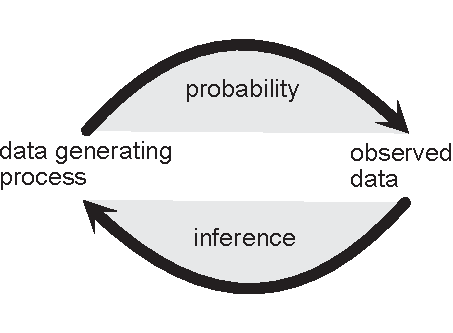
\includegraphics[width=.55\textwidth]{img/probability-inference.pdf}}

\tiny

Wasserman, \emph{All of Statistics} (2003)

\vfill

\normalsize

As long as you can write out the probability\ldots{}
\end{frame}

\begin{frame}{}
\protect\phantomsection\label{section-2}
\end{frame}

\begin{frame}{Central question: How did we get our data?}
\protect\phantomsection\label{central-question-how-did-we-get-our-data}
\Large

\begin{enumerate}
\item
  \textbf{Write down your data generating model}
\item
  Inference: Fit observed data to the model
\item
  Validation: How well? How significant?
\end{enumerate}
\end{frame}

\begin{frame}{Example: the number of mutations in HIV (\texttt{lect02})}
\protect\phantomsection\label{example-the-number-of-mutations-in-hiv-lect02}
\begin{columns}[T]
\begin{column}{.55\linewidth}
Let's graphically represent

\[X \mid \lambda \sim \text{Poisson}(\lambda)\]

where

\begin{itemize}
\item
  \(\lambda\): unknown mutation rate parameter (open)
\item
  \(X\): observed number of mutations (shaded)
\end{itemize}
\end{column}

\begin{column}{.35\linewidth}
\begin{center}
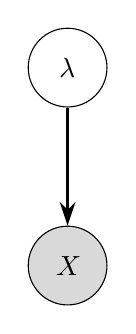
\begin{tikzpicture}[
    node distance=1.5cm,
    observed/.style={circle, draw, fill=gray!30, minimum size=1cm},
    latent/.style={circle, draw, minimum size=1cm},
    param/.style={circle, draw, fill=black, minimum size=0.2cm}
]
\node[latent] (lambda) {$\lambda$};
\node[observed, below=of lambda] (x) {$X$};

\draw[->, thick] (lambda) -- (x);
\end{tikzpicture}
\end{center}
\end{column}
\end{columns}
\end{frame}

\begin{frame}{Revisit the same question: cell type identification}
\protect\phantomsection\label{revisit-the-same-question-cell-type-identification}
\textbf{Data}: RNA-seq of \textbf{genes \(\times\) cells}

\large

Let \(X_{gi}\) be the expression value of a gene \(g\) in a cell \(i\).

\[
\mathbf{X} = \begin{pmatrix}
X_{11} & X_{12} & \cdots & X_{1n} \\
X_{21} & X_{22} & \cdots & X_{2n} \\
\vdots & \vdots & \ddots & \vdots \\
X_{m1} & X_{m2} & \cdots & X_{mn}
\end{pmatrix}
=
\left(
\mathbf{x}_{1}, \mathbf{x}_{2}, \ldots, \mathbf{x}_{n}
\right)\] where \(m\) corresponds to 19k genes.
\end{frame}

\begin{frame}{The number of mRNA counts in the same way?}
\protect\phantomsection\label{the-number-of-mrna-counts-in-the-same-way}
\begin{columns}[T]
\begin{column}{.55\linewidth}
Let's graphically represent

\[X_{gi} \mid \lambda \sim \text{Poisson}(\lambda_{gi})\]

where

\begin{itemize}
\item
  \(\lambda_{gi}\): unknown transcription rate parameter of a gene \(g\)
  within a cell \(i\) (open; latent; parameter)
\item
  \(X_{gi}\): the number of mRNA reads of a gene \(g\) in a cell \(i\)
  (shaded; observed; data)
\end{itemize}
\end{column}

\begin{column}{.35\linewidth}
\begin{center}
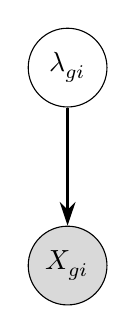
\begin{tikzpicture}[
    node distance=1.5cm,
    observed/.style={circle, draw, fill=gray!30, minimum size=1cm},
    latent/.style={circle, draw, minimum size=1cm},
    param/.style={circle, draw, fill=black, minimum size=0.2cm}
]
\node[latent] (lambda) {$\lambda_{gi}$};
\node[observed, below=of lambda] (x) {$X_{gi}$};

\draw[->, thick] (lambda) -- (x);
\end{tikzpicture}
\end{center}
\end{column}
\end{columns}
\end{frame}

\begin{frame}{Can we elaborate more on the \(\lambda_{gi}\) (gene
\(\times\) cell)?}
\protect\phantomsection\label{can-we-elaborate-more-on-the-lambda_gi-gene-times-cell}
\begin{center}
\includegraphics{../Fig/lect03-problem-formulation/unnamed-chunk-28-1} \end{center}

\vfill

What's wrong with having \(\lambda_{gi}\) for each \(X_{gi}\)?
\end{frame}

\begin{frame}{Let's think of the ``generation'' of \(X\) (or
\(\lambda\))}
\protect\phantomsection\label{lets-think-of-the-generation-of-x-or-lambda}
HINT (just sorted rows and columns):

\begin{center}
\includegraphics{../Fig/lect03-problem-formulation/unnamed-chunk-30-1} \end{center}
\end{frame}

\begin{frame}{Write out data generating scheme}
\protect\phantomsection\label{write-out-data-generating-scheme}
\begin{columns}[T]
\begin{column}{.45\linewidth}
\large

\onslide<1->{Of the $K$ cell types:

$$Z_{ik} = 1 \iff \text{cell $i$ in type $k$}$$

}

\onslide<2->{
For each cell type $k$, a gene $g$ is expressed with the rate

$$\lambda_{gk}$$

*Note*: do we have more $\lambda_{gi}$'s or $\lambda_{gk}$'s?
}

\normalsize
\end{column}

\begin{column}{.45\linewidth}
\large

\onslide<3->{
Given the cell type assignment $Z_{ik}$ and type specific expression rate parameters $\lambda$, we have

$$X_{gi} | Z_{ik}=1 \sim \mathsf{Poisson}(\lambda_{gk})$$
}

\normalsize
\end{column}
\end{columns}
\end{frame}

\begin{frame}{Or we could simply draw it out}
\protect\phantomsection\label{or-we-could-simply-draw-it-out}
\large

\begin{center}
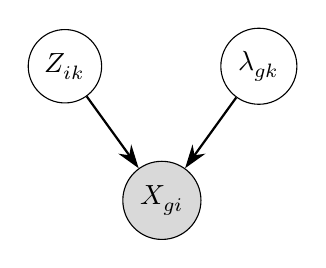
\begin{tikzpicture}[
    node distance=1.2cm,
    observed/.style={circle, draw, fill=gray!30, minimum size=0.9cm},
    latent/.style={circle, draw, minimum size=0.9cm}
]
\node[latent] (z) {$Z_{ik}$};
\node[latent, right=1.5cm of z] (lambda) {$\lambda_{gk}$};
\node[observed, below=1.2cm of $(z)!0.5!(lambda)$] (x) {$X_{gi}$};

\draw[->, thick] (z) -- (x);
\draw[->, thick] (lambda) -- (x);
\end{tikzpicture}
\end{center}

What's next?
\end{frame}

\begin{frame}{Where do these \(Z\) and \(\lambda\) variables correspond
to?}
\protect\phantomsection\label{where-do-these-z-and-lambda-variables-correspond-to}
\begin{columns}[T]
\begin{column}{.1\linewidth}
\end{column}

\begin{column}{.85\linewidth}
\onslide<2>{\large $Z_{ik} \to \to \to$}
\end{column}
\end{columns}

\begin{columns}[T]
\begin{column}{.1\linewidth}
\onslide<2>{\large
\begin{align*}
\lambda_{gk} \\
\downarrow \\
\downarrow
\end{align*}
}
\end{column}

\begin{column}{.85\linewidth}
\begin{center}
\includegraphics{../Fig/lect03-problem-formulation/unnamed-chunk-31-1} \end{center}
\end{column}
\end{columns}
\end{frame}

\begin{frame}[fragile]{In many cases we have assignment \(Z\)
observed/given}
\protect\phantomsection\label{in-many-cases-we-have-assignment-z-observedgiven}
\large

\begin{center}
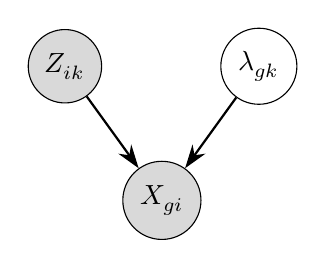
\begin{tikzpicture}[
    node distance=1.2cm,
    observed/.style={circle, draw, fill=gray!30, minimum size=0.9cm},
    latent/.style={circle, draw, minimum size=0.9cm}
]
\node[observed] (z) {$Z_{ik}$};
\node[latent, right=1.5cm of z] (lambda) {$\lambda_{gk}$};
\node[observed, below=1.2cm of $(z)!0.5!(lambda)$] (x) {$X_{gi}$};

\draw[->, thick] (z) -- (x);
\draw[->, thick] (lambda) -- (x);
\end{tikzpicture}
\end{center}

What's next (\texttt{lect04})?

\[\lambda_{g1} = \lambda_{g2} \quad 
\text{or} \quad \lambda_{g1} \neq \lambda_{g2}\]
\end{frame}

\begin{frame}{As long as we have PGM\ldots{}}
\protect\phantomsection\label{as-long-as-we-have-pgm}
\large

\begin{itemize}
\item
  Estimate the unknown parameter, such as \(\lambda\)
\item
  Check how ``well'' generated data, such as \(X\), can explain observed
  \(X\)
\end{itemize}
\end{frame}

\begin{frame}{Summary}
\protect\phantomsection\label{summary}
\large

\textbf{Two approaches to formulate computational problems:}

\normalsize

\begin{columns}[T]
\begin{column}{.45\linewidth}
\begin{enumerate}
\tightlist
\item
  \textbf{Optimization approach}

  \begin{itemize}
  \tightlist
  \item
    Define input, output, metric
  \item
    The art of abstraction
  \item
    Example: MST for cell trajectories
  \end{itemize}
\end{enumerate}
\end{column}

\begin{column}{.45\linewidth}
\begin{enumerate}
\setcounter{enumi}{1}
\tightlist
\item
  \textbf{Probabilistic modeling}

  \begin{itemize}
  \tightlist
  \item
    Write down generative model
  \item
    Use graphical models (PGM)
  \item
    Example: Poisson model for gene expression
  \end{itemize}
\end{enumerate}
\end{column}
\end{columns}

\vfill

\large

\textbf{Key takeaway:} Write down your problem clearly before coding!
\end{frame}

\end{document}
